% Options for packages loaded elsewhere
\PassOptionsToPackage{unicode}{hyperref}
\PassOptionsToPackage{hyphens}{url}
\PassOptionsToPackage{dvipsnames,svgnames,x11names}{xcolor}
%
\documentclass[
  chapter,a4paper,showtrims,openright,hidelinks]{oblivoir}

\usepackage{amsmath,amssymb}
\usepackage{iftex}
\ifPDFTeX
  \usepackage[T1]{fontenc}
  \usepackage[utf8]{inputenc}
  \usepackage{textcomp} % provide euro and other symbols
\else % if luatex or xetex
  \usepackage{unicode-math}
  \defaultfontfeatures{Scale=MatchLowercase}
  \defaultfontfeatures[\rmfamily]{Ligatures=TeX,Scale=1}
\fi
\usepackage{lmodern}
\ifPDFTeX\else  
    % xetex/luatex font selection
\fi
% Use upquote if available, for straight quotes in verbatim environments
\IfFileExists{upquote.sty}{\usepackage{upquote}}{}
\IfFileExists{microtype.sty}{% use microtype if available
  \usepackage[]{microtype}
  \UseMicrotypeSet[protrusion]{basicmath} % disable protrusion for tt fonts
}{}
\makeatletter
\@ifundefined{KOMAClassName}{% if non-KOMA class
  \IfFileExists{parskip.sty}{%
    \usepackage{parskip}
  }{% else
    \setlength{\parindent}{0pt}
    \setlength{\parskip}{6pt plus 2pt minus 1pt}}
}{% if KOMA class
  \KOMAoptions{parskip=half}}
\makeatother
\usepackage{xcolor}
\setlength{\emergencystretch}{3em} % prevent overfull lines
\setcounter{secnumdepth}{5}
% Make \paragraph and \subparagraph free-standing
\ifx\paragraph\undefined\else
  \let\oldparagraph\paragraph
  \renewcommand{\paragraph}[1]{\oldparagraph{#1}\mbox{}}
\fi
\ifx\subparagraph\undefined\else
  \let\oldsubparagraph\subparagraph
  \renewcommand{\subparagraph}[1]{\oldsubparagraph{#1}\mbox{}}
\fi

\usepackage{color}
\usepackage{fancyvrb}
\newcommand{\VerbBar}{|}
\newcommand{\VERB}{\Verb[commandchars=\\\{\}]}
\DefineVerbatimEnvironment{Highlighting}{Verbatim}{commandchars=\\\{\}}
% Add ',fontsize=\small' for more characters per line
\usepackage{framed}
\definecolor{shadecolor}{RGB}{241,243,245}
\newenvironment{Shaded}{\begin{snugshade}}{\end{snugshade}}
\newcommand{\AlertTok}[1]{\textcolor[rgb]{0.68,0.00,0.00}{#1}}
\newcommand{\AnnotationTok}[1]{\textcolor[rgb]{0.37,0.37,0.37}{#1}}
\newcommand{\AttributeTok}[1]{\textcolor[rgb]{0.40,0.45,0.13}{#1}}
\newcommand{\BaseNTok}[1]{\textcolor[rgb]{0.68,0.00,0.00}{#1}}
\newcommand{\BuiltInTok}[1]{\textcolor[rgb]{0.00,0.23,0.31}{#1}}
\newcommand{\CharTok}[1]{\textcolor[rgb]{0.13,0.47,0.30}{#1}}
\newcommand{\CommentTok}[1]{\textcolor[rgb]{0.37,0.37,0.37}{#1}}
\newcommand{\CommentVarTok}[1]{\textcolor[rgb]{0.37,0.37,0.37}{\textit{#1}}}
\newcommand{\ConstantTok}[1]{\textcolor[rgb]{0.56,0.35,0.01}{#1}}
\newcommand{\ControlFlowTok}[1]{\textcolor[rgb]{0.00,0.23,0.31}{#1}}
\newcommand{\DataTypeTok}[1]{\textcolor[rgb]{0.68,0.00,0.00}{#1}}
\newcommand{\DecValTok}[1]{\textcolor[rgb]{0.68,0.00,0.00}{#1}}
\newcommand{\DocumentationTok}[1]{\textcolor[rgb]{0.37,0.37,0.37}{\textit{#1}}}
\newcommand{\ErrorTok}[1]{\textcolor[rgb]{0.68,0.00,0.00}{#1}}
\newcommand{\ExtensionTok}[1]{\textcolor[rgb]{0.00,0.23,0.31}{#1}}
\newcommand{\FloatTok}[1]{\textcolor[rgb]{0.68,0.00,0.00}{#1}}
\newcommand{\FunctionTok}[1]{\textcolor[rgb]{0.28,0.35,0.67}{#1}}
\newcommand{\ImportTok}[1]{\textcolor[rgb]{0.00,0.46,0.62}{#1}}
\newcommand{\InformationTok}[1]{\textcolor[rgb]{0.37,0.37,0.37}{#1}}
\newcommand{\KeywordTok}[1]{\textcolor[rgb]{0.00,0.23,0.31}{#1}}
\newcommand{\NormalTok}[1]{\textcolor[rgb]{0.00,0.23,0.31}{#1}}
\newcommand{\OperatorTok}[1]{\textcolor[rgb]{0.37,0.37,0.37}{#1}}
\newcommand{\OtherTok}[1]{\textcolor[rgb]{0.00,0.23,0.31}{#1}}
\newcommand{\PreprocessorTok}[1]{\textcolor[rgb]{0.68,0.00,0.00}{#1}}
\newcommand{\RegionMarkerTok}[1]{\textcolor[rgb]{0.00,0.23,0.31}{#1}}
\newcommand{\SpecialCharTok}[1]{\textcolor[rgb]{0.37,0.37,0.37}{#1}}
\newcommand{\SpecialStringTok}[1]{\textcolor[rgb]{0.13,0.47,0.30}{#1}}
\newcommand{\StringTok}[1]{\textcolor[rgb]{0.13,0.47,0.30}{#1}}
\newcommand{\VariableTok}[1]{\textcolor[rgb]{0.07,0.07,0.07}{#1}}
\newcommand{\VerbatimStringTok}[1]{\textcolor[rgb]{0.13,0.47,0.30}{#1}}
\newcommand{\WarningTok}[1]{\textcolor[rgb]{0.37,0.37,0.37}{\textit{#1}}}

\providecommand{\tightlist}{%
  \setlength{\itemsep}{0pt}\setlength{\parskip}{0pt}}\usepackage{longtable,booktabs,array}
\usepackage{calc} % for calculating minipage widths
% Correct order of tables after \paragraph or \subparagraph
\usepackage{etoolbox}
\makeatletter
\patchcmd\longtable{\par}{\if@noskipsec\mbox{}\fi\par}{}{}
\makeatother
% Allow footnotes in longtable head/foot
\IfFileExists{footnotehyper.sty}{\usepackage{footnotehyper}}{\usepackage{footnote}}
\makesavenoteenv{longtable}
\usepackage{graphicx}
\makeatletter
\def\maxwidth{\ifdim\Gin@nat@width>\linewidth\linewidth\else\Gin@nat@width\fi}
\def\maxheight{\ifdim\Gin@nat@height>\textheight\textheight\else\Gin@nat@height\fi}
\makeatother
% Scale images if necessary, so that they will not overflow the page
% margins by default, and it is still possible to overwrite the defaults
% using explicit options in \includegraphics[width, height, ...]{}
\setkeys{Gin}{width=\maxwidth,height=\maxheight,keepaspectratio}
% Set default figure placement to htbp
\makeatletter
\def\fps@figure{htbp}
\makeatother

\usepackage{sampl}
\usepackage{kpfonts}
%%%% fonts
\setmainfont{STIX Two Text}
\setsansfont{TeX Gyre Heros}
\setkomainfont(KoPubBatang Light)(KoPubBatang Bold)(KoPubDotum Light)[Scale=MatchUppercase]
\setkosansfont(KoPubDotum Light)(KoPubDotum Bold)(KoPubDotum Medium)[Scale=MatchUppercase]
\newfontfamily\fallbackhanjafont{Noto Serif KR}[Scale=.9]
\setkomonofont{FreeMono}
\chapterstyle{demo}
\AtBeginDocument{\frontmatter}
\DefineVerbatimEnvironment{Highlighting}{Verbatim}{commandchars=\\\{\},baselinestretch=1.1}
\makeindex
\makeatletter
\makeatother
\makeatletter
\makeatother
\makeatletter
\@ifpackageloaded{caption}{}{\usepackage{caption}}
\AtBeginDocument{%
\ifdefined\contentsname
  \renewcommand*\contentsname{목 차}
\else
  \newcommand\contentsname{목 차}
\fi
\ifdefined\listfigurename
  \renewcommand*\listfigurename{List of Figures}
\else
  \newcommand\listfigurename{List of Figures}
\fi
\ifdefined\listtablename
  \renewcommand*\listtablename{List of Tables}
\else
  \newcommand\listtablename{List of Tables}
\fi
\ifdefined\figurename
  \renewcommand*\figurename{그림}
\else
  \newcommand\figurename{그림}
\fi
\ifdefined\tablename
  \renewcommand*\tablename{Table}
\else
  \newcommand\tablename{Table}
\fi
}
\@ifpackageloaded{float}{}{\usepackage{float}}
\floatstyle{ruled}
\@ifundefined{c@chapter}{\newfloat{codelisting}{h}{lop}}{\newfloat{codelisting}{h}{lop}[chapter]}
\floatname{codelisting}{Listing}
\newcommand*\listoflistings{\listof{codelisting}{List of Listings}}
\makeatother
\makeatletter
\@ifpackageloaded{caption}{}{\usepackage{caption}}
\@ifpackageloaded{subcaption}{}{\usepackage{subcaption}}
\makeatother
\makeatletter
\makeatother
\ifLuaTeX
  \usepackage{selnolig}  % disable illegal ligatures
\fi
\usepackage[]{biblatex}
\addbibresource{sample.bib}
\IfFileExists{bookmark.sty}{\usepackage{bookmark}}{\usepackage{hyperref}}
\IfFileExists{xurl.sty}{\usepackage{xurl}}{} % add URL line breaks if available
\urlstyle{same} % disable monospaced font for URLs
\hypersetup{
  pdftitle={중심극한정리(Central Limit Theorem)의 예시},
  pdfauthor={한글 텍 사용자 그룹},
  colorlinks=true,
  linkcolor={blue},
  filecolor={Maroon},
  citecolor={Blue},
  urlcolor={Blue},
  pdfcreator={LaTeX via pandoc}}

\title{중심극한정리(Central Limit Theorem)의 예시}
\author{한글 텍 사용자 그룹}
\date{2023-08-10}

\begin{document}
\maketitle
\renewcommand*\contentsname{목 차}
{
\hypersetup{linkcolor=}
\setcounter{tocdepth}{2}
\tableofcontents
}
\mainmatter
\pagestyle{demo}

\hypertarget{uxc911uxc2ecuxadf9uxd55cuxc815uxb9ac}{%
\chapter{중심극한정리}\label{uxc911uxc2ecuxadf9uxd55cuxc815uxb9ac}}

상자 안에 1에서 999까지 숫자가 표시된 999개의 상태가 균질한 공(\(X\))을
넣고 이를 특정한 모집단(population)이라고
가정하자.\index{모집단}\index{상자} 이 모집단의 평균 \(\mu\)은
500이다.\index{평균} 모집단의 분산 \(\mathrm{var}(X)\)는
80,475이다.\index{분산}

이 중 30개의 공을 50회에 걸쳐 반복 추출한다.\index{반복 추출} 이 경우
표본평균의 분포는 \(E(\bar{X}_i)=\mu(X)\)이고 분산이
\(\mathrm{var}(\bar{X_i})=\frac{\sigma^2}{n}\)인 정규분포에 근사한다.
즉, \(X \sim \mathcal{N}(500,~283.7^2)\)이다.\index{근사}

\hypertarget{uxc2e4uxd5d8}{%
\chapter{실험}\label{uxc2e4uxd5d8}}

\hypertarget{uxc774uxb97c-uxc2e4uxd5d8uxc744-uxd1b5uxd574-uxc0b4uxd3b4uxbcf4uxc790.}{%
\section{이를 실험을 통해
살펴보자.}\label{uxc774uxb97c-uxc2e4uxd5d8uxc744-uxd1b5uxd574-uxc0b4uxd3b4uxbcf4uxc790.}}

999개의 공이 든 상자에서 30개의 공을 50회에 걸쳐 무작위
반복추출하고(30개의 공을 뽑은 뒤, 다시 그 공을 상자 안에 집어 놓고
상자를 처음과 같은 상태가 되도록 뒤흔들어서 다시 30개의 공을 뽑는 것을
50회 반복한다), 그 각각의 평균을 기록하면 다음과
같다.\index{실험}\index{반복}

\begin{quote}
\begin{quote}
\textbf{50회 반복추출의 평균값:} 444.0, 535.6, 551.0, 547.0, 598.4,
465.0, 458.7, 483.8, 460.6, 597.9, 561.4, 512.6, 446.3, 539.1, 573.3,
498.1, 452.7, 496.7, 501.0, 513.4, 442.9, 531.1, 487.3, 512.1, 549.1,
492.8, 487.2, 512.8, 469.6, 409.0, 464.6, 604.1, 507.4, 558.0, 531.6,
465.3, 475.2, 586.6, 553.8, 454.3, 534.8, 419.2, 497.0, 470.6, 465.5,
426.4, 519.7, 429.7, 522.8, 503.0
\end{quote}
\end{quote}

표본평균값의 분포를 히스토그램으로 표현하면 그림~\ref{fig-test}와
같다.\sidepar{\sffamily\small여기서 자동조사가 잘 구현되는지 확인하라. 소스는 ``와 같다''로 되어 있으나 ``과 같다''라고 인쇄되어야 한다.}\index{히스토그램}

\begin{figure}

{\centering 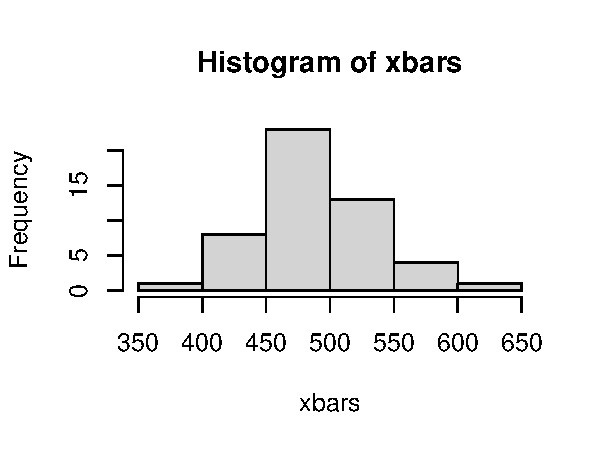
\includegraphics{clt_files/figure-pdf/fig-test-1.pdf}

}

\caption{\label{fig-test}표본평균의 히스토그램}

\end{figure}

\hypertarget{uxadf8uxb9bcuxc5d0uxc11c-uxbcf4uxb4ef}{%
\section{그림에서 보듯}\label{uxadf8uxb9bcuxc5d0uxc11c-uxbcf4uxb4ef}}

\(\bar{X_i}\)는 500을 중심으로 좌우대칭적으로 분포하고 있다.
\sidepar{이 텍스트는 사이드노트를 시험하기 위한 것이다.}\index{자동조사}
이들의 평균은 502.4으로 모평균 500과
근사하다.\index{근사}\index{좌우대칭} 이들 중 이론적으로 산출한
평균으로부터 약 2 표준편차만큼 떨어진
구간(\(\mu \pm 2\frac{\sigma}{\sqrt{n}}\)) 안에 속하는 값, 즉
\([396.4, 603.6]\)의 범위 안에 있는 값의 개수를 세면 모두
49개이다.\index{표준편차}

표본평균 분포의 약 95\%를 포괄하고 있음을 알 수
있다.\index{분포}\index{표본평균}

\hypertarget{r-markdown}{%
\section{R Markdown}\label{r-markdown}}

\textbf{Render} 버튼을 누르면 문서가 생성된다. 여기에는 내용과 함께
내장된 R 코드 청크가 실행된다. R 코드는 다음과 같이 포함할 수
있다.\index{문서 생성}\index{코드}

\begin{Shaded}
\begin{Highlighting}[]
\FunctionTok{summary}\NormalTok{(cars)}
\end{Highlighting}
\end{Shaded}

\begin{verbatim}
     speed           dist       
 Min.   : 4.0   Min.   :  2.00  
 1st Qu.:12.0   1st Qu.: 26.00  
 Median :15.0   Median : 36.00  
 Mean   :15.4   Mean   : 42.98  
 3rd Qu.:19.0   3rd Qu.: 56.00  
 Max.   :25.0   Max.   :120.00  
\end{verbatim}

\hypertarget{uxd50cuxb85cuxd2b8-uxd3ecuxd568uxd558uxae30}{%
\section{플로트
포함하기}\label{uxd50cuxb85cuxd2b8-uxd3ecuxd568uxd558uxae30}}

플로트도 포함할 수 있으니, 다음과 같다.\index{플로트}

\begin{figure}

{\centering 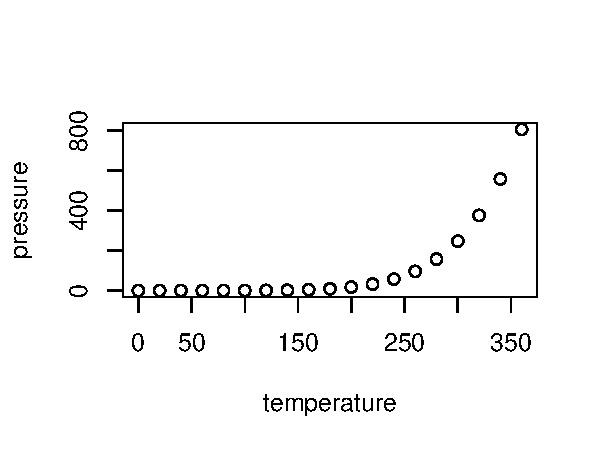
\includegraphics{clt_files/figure-pdf/fig-test2-1.pdf}

}

\caption{\label{fig-test2}Pressure}

\end{figure}

\texttt{echo\ =\ FALSE} 파라미터를 주었기 때문에 이 플로트를 생성하는 R
코드가 인쇄되지 않는다. 그림~\ref{fig-test2}을
보자.\index{파라미터}\index{인쇄}

\hypertarget{uxc7acuxbbf8uxc788uxb294-uxbc30uxc5f4-uxbb38uxc81c}{%
\section{재미있는 배열
문제}\label{uxc7acuxbbf8uxc788uxb294-uxbc30uxc5f4-uxbb38uxc81c}}

\begin{Shaded}
\begin{Highlighting}[]
\NormalTok{N, C }\OperatorTok{=} \DecValTok{13}\NormalTok{,}\DecValTok{3}
\NormalTok{a}\OperatorTok{=}\NormalTok{[ }\SpecialStringTok{f"}\SpecialCharTok{\{}\NormalTok{i}\OperatorTok{+}\DecValTok{1}\SpecialCharTok{\}}\SpecialStringTok{"} \ControlFlowTok{for}\NormalTok{ i }\KeywordTok{in} \BuiltInTok{range}\NormalTok{(N) ]}
\ControlFlowTok{for}\NormalTok{ i }\KeywordTok{in} \BuiltInTok{range}\NormalTok{(}\DecValTok{1}\NormalTok{, C):}
    \ControlFlowTok{if} \BuiltInTok{len}\NormalTok{(a)}\OperatorTok{\%}\NormalTok{C }\OperatorTok{==}\NormalTok{ i: a.insert((}\BuiltInTok{len}\NormalTok{(a)}\OperatorTok{//}\NormalTok{C}\OperatorTok{+}\DecValTok{1}\NormalTok{)}\OperatorTok{*}\NormalTok{(i}\OperatorTok{+}\DecValTok{1}\NormalTok{)}\OperatorTok{{-}}\DecValTok{1}\NormalTok{, }\StringTok{" "}\NormalTok{)}
\BuiltInTok{print}\NormalTok{(}\StringTok{"}\CharTok{\textbackslash{}\textbackslash{}}\StringTok{begin}\SpecialCharTok{\{tabular\}}\StringTok{\{}\SpecialCharTok{\%s}\StringTok{\}"}\OperatorTok{\%}\NormalTok{(}\StringTok{"l"}\OperatorTok{*}\NormalTok{C))}
\end{Highlighting}
\end{Shaded}

\begin{verbatim}
\begin{tabular}{lll}
\end{verbatim}

\begin{Shaded}
\begin{Highlighting}[]
\ControlFlowTok{for}\NormalTok{ i }\KeywordTok{in} \BuiltInTok{range}\NormalTok{(}\BuiltInTok{len}\NormalTok{(a)}\OperatorTok{//}\NormalTok{C): }\BuiltInTok{print}\NormalTok{(}\StringTok{" \& "}\NormalTok{.join(a[i::}\BuiltInTok{len}\NormalTok{(a)}\OperatorTok{//}\NormalTok{C]), }\StringTok{" }\CharTok{\textbackslash{}\textbackslash{}\textbackslash{}\textbackslash{}}\StringTok{"}\NormalTok{)}
\end{Highlighting}
\end{Shaded}

\begin{verbatim}
1 & 6 & 10  \\
2 & 7 & 11  \\
3 & 8 & 12  \\
4 & 9 & 13  \\
5 &   &    \\
\end{verbatim}

\begin{Shaded}
\begin{Highlighting}[]
\BuiltInTok{print}\NormalTok{(}\StringTok{"}\CharTok{\textbackslash{}\textbackslash{}}\StringTok{end}\SpecialCharTok{\{tabular\}}\StringTok{"}\NormalTok{)}
\end{Highlighting}
\end{Shaded}

\begin{verbatim}
\end{tabular}
\end{verbatim}

이 문제는 흥미롭다. KTUG 게시판에 올라온 문제에 대하여 aud라는 분이 단
답변이다. 한편 \textsc{Expl3}로도 같은 일을 할 수 있음이 답글 중에
제시되어 있다.\index{케이턱@KTUG}

\hypertarget{tabularuxc640-bibliography}{%
\chapter{tabular와 bibliography}\label{tabularuxc640-bibliography}}

\hypertarget{uxac1cuxad00}{%
\section{개관}\label{uxac1cuxad00}}

Quarto의 특징 중의 하나는 \LaTeX~문서의 소스를 그대로 집어넣어도 된다는
것이다. 이 장의 텍스트는 다른 곳에서 작성한 \TeX~소스를 복사한 것이다.
\index{Quarto}\index{LaTeX@\LaTeX}

\hypertarget{uxd45c-uxadf8uxb9acuxae30}{%
\section{표 그리기}\label{uxd45c-uxadf8uxb9acuxae30}}

다른 곳에서 책을 하나 조판하던 때에, tabular의 괘선에 색을 입혀달라는
요구가 있었다.\index{tabular} 2020년경이었는데, 당시로서 이것을 구현하는
것은 거의 불가능해 보였으나 어찌어찌 tabular 자체 코드를 해킹해서
어렵사리 성공했더랬다. 그리고 잠시 지났더니 \pkg{tabularray}가 나왔다.
조금 더 일찍 나왔다면 그 고생을 하지 않았을 것 아닌가!\index{tabularray}

\begin{margintable}
\centering
\caption{색깔 있는 괘선}
\begin{tblr}{
    colspec = {ccc},
    hlines = {blue},
    vlines = {red}
}
a & b & c \\
1 & 2 & 3
\end{tblr}
\end{margintable}

\begin{code}
\begin{tblr}{
    colspec = {ccc},
    hlines = {blue},
    vlines = {red}
}
a & b & c \\
1 & 2 & 3
\end{tblr}
\end{code}

이 패키지를 사용하면 그동안 골칫거리였던 tabular 관련 문제가 대부분
해결된다. 사용법이 조금 복잡해보일지 모르지만 익숙해지면 편하게 쓸 수
있다.

\hypertarget{footnotes-in-boxed-environment}{%
\section{footnotes in boxed
environment}\label{footnotes-in-boxed-environment}}

\LaTeX 의 apparatus 중에 minipage footnote라는 것이 있다. 예를 들면
다음과 같은 것이다.

\bigskip

\begin{minipage}{.5\textwidth}
미니페이지 안에서는 각주\footnote{미니페이지 안의 각주}가
조금 다른 모양으로 붙는다.
\end{minipage}

\medskip

이것은 매우 유용한 장치이기는 하나, 단행본을 출간하는 입장에서 가끔 모든
각주를 페이지 하단에 넣으라는 요구를 받을 때가 있다. 가장 간단한
해결책은 \cs{footnote} 명령을 \cs{footnotemark}와 \cs{footnotetext}로
분해하는 것이다.

\hypertarget{uxbb38uxd5ccuxbaa9uxb85d}{%
\section{문헌목록}\label{uxbb38uxd5ccuxbaa9uxb85d}}

참고 문헌 인용과 목록 생성 실험을
합니다.\index{참고 문헌}\index{인용}\index{citation} 한국어 문헌과
구미어 문헌은 그 목록형성과 인용 방법이 다릅니다. 한국어 문헌의 예를
들면, \autocite{kimuycwung_hankwukphan_2003}\과 같고, 영어 문헌은 예를
들면, \autocite{Allport:1992:OND}\과 같습니다.
\index{타당도}\index{신뢰도}\index{한국어 문헌}\index{korean}

\backmatter


\printbibliography


\printindex

\end{document}
